\documentclass{beamer}

% To have the citation lists ordered by number.
\usepackage[nocompress]{cite}
\usepackage[utf8]{inputenc}
\usepackage{graphicx}
\usepackage[tight,TABTOPCAP]{subfigure}
\usepackage{amsmath}
\usepackage{amssymb}
\usepackage{amsfonts}
\usepackage{url}

\usepackage{hyperref}

\usepackage{tikz}
\usepackage{color}
\usetikzlibrary{automata,backgrounds,petri}

% Allow more than 70% (default) of a page to be filled by figures (100%).
\renewcommand\topfraction{1.0}

%%%%%%%%%% Tool Names %%%%%%%%%%%%
\newcommand{\csisat}{{\sc CSIsat}}
\newcommand{\blast}{{\sc Blast}}
\newcommand{\armc}{{\sc ARMC}}
\newcommand{\mathsat}{{\sc MathSAT}}
\newcommand{\picosat}{{\sc PicoSAT}}
\newcommand{\clpprover}{{\sc CLPprover}}
\newcommand{\foci}{{\sc Foci}}
\newcommand{\sicstus}{{\sc SICStus Prolog}}
\newcommand{\scala}{\textsc{Scala}}

\mode<presentation>
{
  \usetheme{Warsaw}
  \useoutertheme{mysplit}
}
% Remove the navigation bar
\setbeamertemplate{navigation symbols}{}

\graphicspath{{./imgs/}}

\title[Verifying actors]{Modeling and verifying \scala{} actors}

\AtBeginSection[]
{
  \begin{frame}<beamer>
    \frametitle{Outline}
    \tableofcontents[currentsection]
  \end{frame}
}

\author{ Damien Zufferey}

\institute{
  \'Ecole Polytechnique F\'ed\'erale de Lausanne
}
\date{\today}

%-------------------------------------------------------------------------
\begin{document}

% Title
%\frame[plain]{\titlepage}
\begin{frame}[plain]
%\titlepage
\begin{center}

{\Large
\inserttitle
}

\vspace{10mm}

\insertauthor

\vspace{5mm}

{\footnotesize
\insertinstitute

\vspace{2mm}

\begin{tabular}{ll}
Laboratory: & Models and Theory of Computation\\
Supervisor: & Tom Henzinger\\
Assistant: & Thomas Wies
\end{tabular}
}

\vspace{8mm}
\small
\today
\end{center}
\end{frame}

\section*{Outline}
\begin{frame}
\tableofcontents
\end{frame}

\section{Introduction}

\subsection{Paradigms for concurrency}

\begin{frame}
  \frametitle{Shared memory}
  
  \begin{columns}
  \column{5cm}
  Communication using a memory that every process can access (read and write).

  \column{5cm}
  \centering
  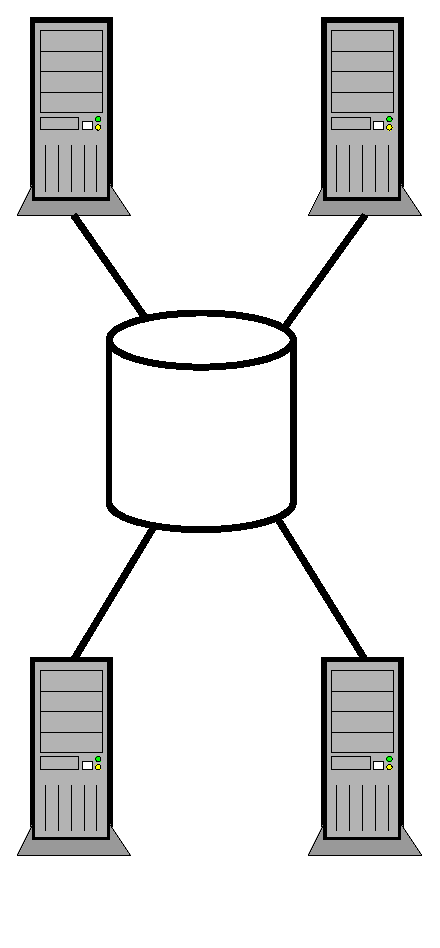
\includegraphics[width=2cm]{shared}
  \end{columns}

  $+$ Fast \\
  $-$ Limited scaling \\
  $-$ Hard to program (deadlocks, races, ...)
\end{frame}

\begin{frame}
  \frametitle{Message passing}
  
  \begin{columns}
  \column{5cm}
  Processes exchange messages.

  \column{5cm}
  \centering
  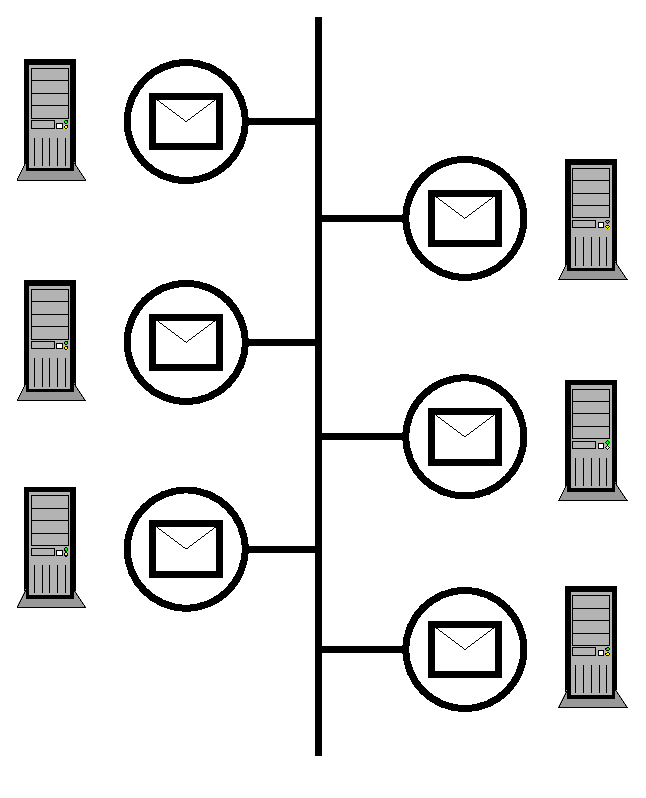
\includegraphics[width=3.5cm]{message}
  \end{columns}

  $+$ Scales well\\
  $-$ Slower \\
  $\sim$ Hard to program (easier than shared memory ?)
\end{frame}

\subsection{Actors in \scala{}}

\begin{frame}[fragile]
  \frametitle{Example (1): scala/docs/examples/actors/pingpong.scala}

  \begin{columns}
    \column{6cm}
{\tiny
\begin{verbatim}
class Ping(count: Int, pong: Actor) extends Actor {
  def act() {
    var pingsLeft = count - 1
    pong ! Ping
    loop {
      react {
        case Pong =>
          if (pingsLeft % 1000 == 0)
            println("Ping: pong")
          if (pingsLeft > 0) {
            pong ! Ping
            pingsLeft -= 1
          } else {
            println("Ping: stop")
            pong ! Stop
            exit()
          }
      }
    }
  }
}
\end{verbatim}
}

    \column{5cm}
{\tiny
\begin{verbatim}
class Pong extends Actor {
  def act() {
    var pongCount = 0
    loop {
      react {
        case Ping =>
          if (pongCount % 1000 == 0)
            println("Pong: ping "+pongCount)
          sender ! Pong
          pongCount += 1
        case Stop =>
          println("Pong: stop")
          exit()
      }
    }
  }
}
\end{verbatim}
}
  \end{columns}
\end{frame}

\begin{frame}[label=cfa]
  \frametitle{Example (2): scala/docs/examples/actors/pingpong.scala}

  \begin{columns}
    \column{5cm}
    \begin{figure}[!ht]
      \centering
      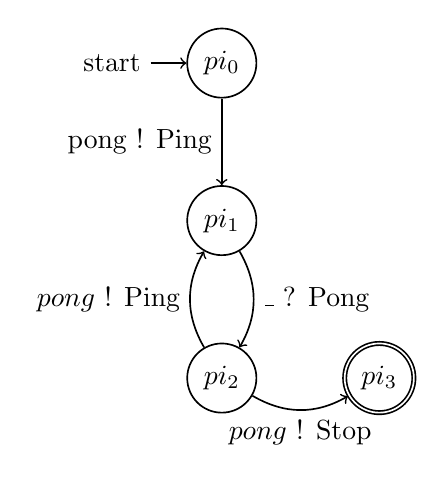
\begin{tikzpicture}[->,auto, node distance=2cm, semithick]
      \node [state,initial] (pi0) {$pi_0$};
      \node [state] (pi1) [below of=pi0] {$pi_1$};
      \node [state] (pi2) [below of=pi1] {$pi_2$};
      \node [state,accepting] (pi3) [right of=pi2] {$pi_3$};
      \path
      (pi0) edge node[left] { pong ! Ping } (pi1)
      (pi1) edge [bend left] node[right] { \_ ? Pong } (pi2)
      (pi2) edge [bend left] node[left] { $pong$ ! Ping } (pi1)
      (pi2) edge [bend right] node[below] { $pong$ ! Stop } (pi3)
      ;
      \end{tikzpicture}
%      \caption{Ping($pong$)}
%      \label{ping}
    \end{figure}

    \column{5cm}
    \begin{figure}[!ht]
      \centering
      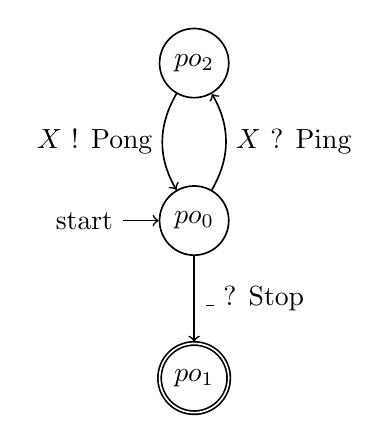
\begin{tikzpicture}[->,auto, node distance=2cm, semithick]
      \node [state,initial] (po0) {$po_0$};
      \node [state,accepting] (po1) [below of=po0] {$po_1$};
      \node [state] (po2) [above of=po0] {$po_2$};
      \path
      (po0) edge node[right] { \_ ? Stop } (po1)
      (po0) edge [bend right] node[right] { $X$ ? Ping } (po2)
      (po2) edge [bend right] node[left] { $X$ ! Pong} (po0)
      ;
      \end{tikzpicture}
%      \caption{Pong}
%      \label{pong}
    \end{figure}
  \end{columns}
\end{frame}


\begin{frame}[label=implementation]
  \frametitle{Overview of Analysis}
  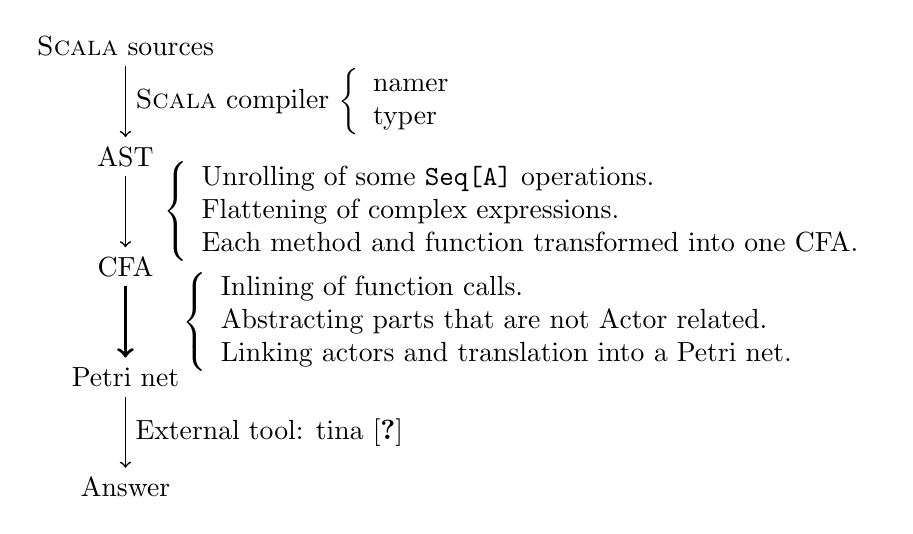
\begin{tikzpicture}[->,auto, node distance=1.4cm, semithick]
    \node (po0) {\scala{} sources};
    \node (po1) [below of=po0] {AST};
    \node (po2) [below of=po1] {CFA};
    \node (po3) [below of=po2] {Petri net};
    \node (po4) [below of=po3] {Answer};
    \path
    (po0) edge node[right] { \scala{} compiler $\left\{ \begin{array}{l} \mbox{namer} \\ \mbox{typer} \end{array} \right.$ } (po1)
    (po1) edge node[right] { ~~ $\left\{ \begin{array}{l}
        \mbox{Unrolling of some \texttt{Seq[A]} operations.} \\
        \mbox{Flattening of complex expressions.} \\
        \mbox{Each method and function transformed into one CFA.}
      \end{array} \right.$ } (po2)
    (po2) edge[very thick] node[right] { ~~~~ $\left\{ \begin{array}{l}
        \mbox{Inlining of function calls.} \\
        \mbox{Abstracting parts that are not Actor related.} \\
        \mbox{Linking actors and translation into a Petri net.} \\
      \end{array} \right.$ } (po3)
    (po3) edge node[right] { External tool: tina\cite{DBLP:conf/qest/BerthomieuV06}} (po4)
    ;
  \end{tikzpicture}
\end{frame}


\section{The Actor Model}

\begin{frame}
  \frametitle{Overview}
  \alt<2>{The \textcolor{red}{Actor Model}\cite{DBLP:conf/ijcai/HewittBS73}}{Object oriented programming}
  uses \emph{\alt<2>{\textcolor{red}{actors}}{objects}} and their interactions
  to build \alt<2>{\textcolor{red}{concurrent} softwares}{software systems}.\\

  \vspace{5pt}

  An \alt<2>{\textcolor{red}{actor}}{object} can:
  \begin{itemize}
  \item receive messages
  \item \alt<2>{\textcolor{red}{create new actors}}{process data}
  \item send messages
  \end{itemize}

  \vspace{10pt}

  \visible<2>{The meaning of messages is not the same in both contexts.}
\end{frame}

\begin{frame}
  \frametitle{Models and decidability}

\begin{tabular}{l|l}
Model & Reachability\\
\hline
\hline
Synchronous & decidable \\
\hline
Asynchronous with queues & undecidable\\
 & \cite{DBLP:journals/jacm/BrandZ83} \\
% many to one or one to one queues & \cite{DBLP:journals/jacm/BrandZ83} \\
\hline
Asynchronous with multisets  & decidable\footnotemark \\
& \cite{DBLP:journals/njc/AmadioM02} \\
\hline
Asynchronous with lossy queues & decidable\footnotemark \\
& \cite{DBLP:journals/iandc/AbdullaJ96} \\
\hline
\end{tabular}

\vspace{20pt}

With recursion, all models are undecidable \cite{DBLP:journals/toplas/Ramalingam00}.

\footnotetext[1]{fixed number of actors}
\footnotetext{undecidable with fair channel \cite{DBLP:journals/iandc/AbdullaJ96a}}

\end{frame}

\begin{frame}
  \frametitle{Chosen model and Assumptions}

  Finite state machines with unordered mailbox (asynchronous).

  \vspace{20pt}

  To preserve decidability, we need to add the following assumptions:
  \begin{itemize}
  \item finite data-types,
  \item no recursion,
  \item no dynamic actor creation.
%  \item static topology.
  \end{itemize}
\end{frame}

\section{$\pi$-calculus and $A\pi$-calculus}

\begin{frame}
\frametitle{What is it ?}
The $\pi$-calculus\cite{DBLP:journals/iandc/MilnerPW92a,DBLP:journals/iandc/MilnerPW92b} is considered to be the $\lambda$-calculus of message-passing concurrency.
It tries to be minimal, but is still able to model complex features:

\begin{itemize}
\item synchronous and asynchronous communication
\item changing topologies
\item dynamic creation of processes and names
\end{itemize}

\vspace{5pt}

The $A\pi$-calculus\cite{DBLP:conf/ecoop/HondaT91,Boudol92asynchronyand} is a restriction of $\pi$-calculus that only allows asynchronous communication.

\end{frame}

\begin{frame}
\frametitle{Grammar}

\begin{tabular}{lclrl}
$P$ & ::= & $x(y).P $                           & input prefix & (receiving messages)\\
    & $|$ & $\overline{x} \langle y \rangle.P $ & output prefix & (sending messages) \\
    & $|$ & $P\;|\;P $                          & parallel composition & \\
    & $|$ & $(\nu x)P $                         & name creation & (names are channels)\\
    & $|$ & $!P $                               & replication & \\
    & $|$ & $0 $                                & unit process & (finished execution)
\end{tabular}

\vspace{1cm}

The only kind of output prefix allowed in $A\pi$-calculus is `$\overline{x} \langle y \rangle.0 $'.

\end{frame}

\begin{frame}
\frametitle{Semantic}

The most important reduction rules:
\begin{equation*}
\overline{x}\langle z \rangle.P \;|\; x(y).Q \rightarrow P \;|\; Q[z/y]
\end{equation*}

\vspace{10pt}

Some congruence rules:
\begin{columns}

\column{5cm}
\begin{itemize}
\item $P\;|\;Q \equiv Q\;|\;P$
\item $P\;|\;0 \equiv P$
\item $(P\;|\;Q)\;|\;R \equiv P\;|\;(Q\;|\;R)$
\end{itemize}

\column{5cm}
\begin{itemize}
\item $(\nu x)(\nu y)P \equiv (\nu y)(\nu x)P$
\item $(\nu x)0 \equiv 0$
\item $!P \equiv P\;|\;!P$
\end{itemize}

\end{columns}
\end{frame}

\begin{frame}
\frametitle{Example}

$
(\nu p_{ing})(\nu p_{ong}) !( \overline{p_{ong}}\langle p_{ing} \rangle. p_{ing}(p_{ong}). 0 )
                     \;|\; !( p_{ong}(p_{ing}). \overline{p_{ing}}\langle p_{ong} \rangle. 0 )
$ \pause \\

\vspace{15pt}

$
(\nu p_{ing})(\nu p_{ong}) !( \overline{p_{ong}}\langle p_{ing} \rangle. p_{ing}(p_{ong}). 0 )
                     \;|\; !( p_{ong}(p_{ing}). \overline{p_{ing}}\langle p_{ong} \rangle. 0 ) $ \\
\hspace{1cm} $       \;|\; \overline{p_{ong}}\langle p_{ing} \rangle. p_{ing}(p_{ong}). 0
                     \;|\; p_{ong}(p_{ing}). \overline{p_{ing}}\langle p_{ong} \rangle. 0 $
\pause \\

\vspace{15pt}

$
(\nu p_{ing})(\nu p_{ong}) !( \overline{p_{ong}}\langle p_{ing} \rangle. p_{ing}(p_{ong}). 0 )
                     \;|\; !( p_{ong}(p_{ing}). \overline{p_{ing}}\langle p_{ong} \rangle. 0 ) $ \\
\hspace{1cm} $       \;|\; p_{ing}(p_{ong}). 0
                     \;|\; \overline{p_{ing}}\langle p_{ong} \rangle. 0 $
\pause \\

\vspace{15pt}

$
(\nu p_{ing})(\nu p_{ong}) !( \overline{p_{ong}}\langle p_{ing} \rangle. p_{ing}(p_{ong}). 0 )
                     \;|\; !( p_{ong}(p_{ing}). \overline{p_{ing}}\langle p_{ong} \rangle. 0 ) $ \\
\hspace{1cm} $       \;|\; 0
                     \;|\; 0 $
\pause \\

\vspace{15pt}

$
(\nu p_{ing})(\nu p_{ong}) !( \overline{p_{ong}}\langle p_{ing} \rangle. p_{ing}(p_{ong}). 0 )
                     \;|\; !( p_{ong}(p_{ing}). \overline{p_{ing}}\langle p_{ong} \rangle. 0 )
$

\end{frame}

\section{Petri nets}

\begin{frame}
\frametitle{Overview}

Petri nets are modeling language for discrete distributed systems.\\

\vspace{10pt}

A Petri net is a directed bipartite graph where the nodes are divided in \emph{places} and \emph{transitions}.\\
Places may contain some tokens, that are consumed and created by transitions.

\end{frame}

\begin{frame}
  \frametitle{Example}

  \begin{columns}
    \column{5cm}
    \begin{figure}[!ht]
      \centering
      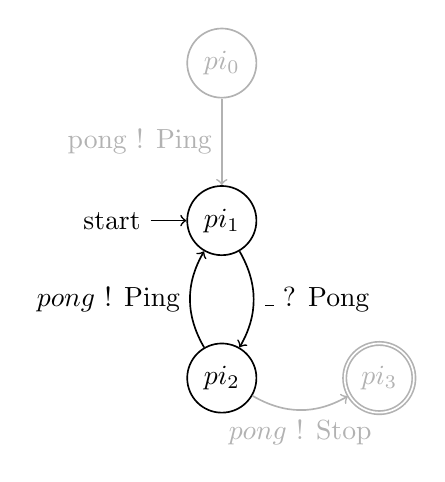
\begin{tikzpicture}[->,auto, node distance=2cm, semithick]
      \node [state,color=black!30] (pi0) {$pi_0$};
      \node [state,initial] (pi1) [below of=pi0] {$pi_1$};
      \node [state] (pi2) [below of=pi1] {$pi_2$};
      \node [state,accepting,color=black!30] (pi3) [right of=pi2] {$pi_3$};
      \path
      (pi0) edge [color=black!30] node[left] { pong ! Ping } (pi1)
      (pi1) edge [bend left] node[right] { \_ ? Pong } (pi2)
      (pi2) edge [bend left] node[left] { $pong$ ! Ping } (pi1)
      (pi2) edge [bend right,color=black!30] node[below] { $pong$ ! Stop } (pi3)
      ;
      \end{tikzpicture}
    \end{figure}

    \column{5cm}
    \begin{figure}[!ht]
      \centering
      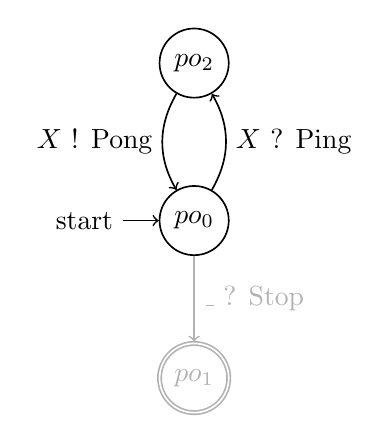
\begin{tikzpicture}[->,auto, node distance=2cm, semithick]
      \node [state,initial] (po0) {$po_0$};
      \node [state,accepting,color=black!30] (po1) [below of=po0] {$po_1$};
      \node [state] (po2) [above of=po0] {$po_2$};
      \path
      (po0) edge [color=black!30] node[right] { \_ ? Stop } (po1)
      (po0) edge [bend right] node[right] { $X$ ? Ping } (po2)
      (po2) edge [bend right] node[left] { $X$ ! Pong} (po0)
      ;
      \end{tikzpicture}
    \end{figure}
  \end{columns}
\end{frame}


\begin{frame}
\frametitle{Example}
\begin{figure}[!ht]
  \centering
  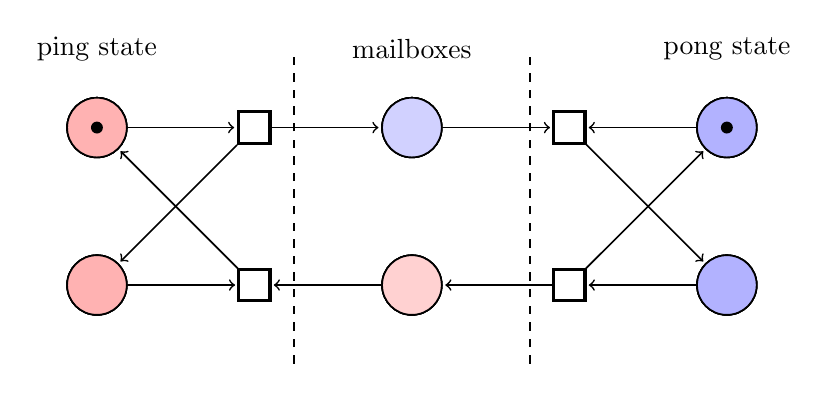
\begin{tikzpicture}[auto, node distance=2cm, semithick]

  \node (label1) at (-4,3) {ping state};
  \node (label2) at ( 0,3) {mailboxes};
  \node (label3) at ( 4,3) {pong state};
  \draw[dashed] (-1.5,-1) -- (-1.5,3);
  \draw[dashed] (1.5,-1) -- (1.5,3);

  \alt<1,5>{
  \node [place,fill=red!18] (ping) at (0,0) {};
  \node [place,tokens=1,fill=blue!18] (pong) [above of= ping] {};

  \node [transition,very thick] (pongCatch) [right of= pong] {};
  \node [transition] (pongSend)  [below of= pongCatch] {};
  \node [place,tokens=1,fill=blue!30] (po0) [right of= pongCatch] {};
  \node [place,fill=blue!30] (po1) [below of= po0] {};
  
  \node [transition] (pingCatch) [left of = ping] {};
  \node [transition] (pingSend) [above of= pingCatch] {};
  \node [place,tokens=1,fill=red!30] (pi0) [left of= pingCatch] {};
  \node [place,fill=red!30] (pi1) [above of= pi0] {};
  }{
  \alt<2>{
  \node [place,fill=red!18] (ping) at (0,0) {};
  \node [place,fill=blue!18] (pong) [above of= ping] {};

  \node [transition] (pongCatch) [right of= pong] {};
  \node [transition,very thick] (pongSend)  [below of= pongCatch] {};
  \node [place,fill=blue!30] (po0) [right of= pongCatch] {};
  \node [place,tokens=1,fill=blue!30] (po1) [below of= po0] {};
  
  \node [transition] (pingCatch) [left of = ping] {};
  \node [transition] (pingSend) [above of= pingCatch] {};
  \node [place,tokens=1,fill=red!30] (pi0) [left of= pingCatch] {};
  \node [place,fill=red!30] (pi1) [above of= pi0] {};
  }{
  \alt<3>{
  \node [place,tokens=1,fill=red!18] (ping) at (0,0) {};
  \node [place,fill=blue!18] (pong) [above of= ping] {};

  \node [transition] (pongCatch) [right of= pong] {};
  \node [transition] (pongSend)  [below of= pongCatch] {};
  \node [place,tokens=1,fill=blue!30] (po0) [right of= pongCatch] {};
  \node [place,fill=blue!30] (po1) [below of= po0] {};
  
  \node [transition,very thick] (pingCatch) [left of = ping] {};
  \node [transition] (pingSend) [above of= pingCatch] {};
  \node [place,tokens=1,fill=red!30] (pi0) [left of= pingCatch] {};
  \node [place,fill=red!30] (pi1) [above of= pi0] {};
  }{
  \node [place,fill=red!18] (ping) at (0,0) {};
  \node [place,fill=blue!18] (pong) [above of= ping] {};

  \node [transition] (pongCatch) [right of= pong] {};
  \node [transition] (pongSend)  [below of= pongCatch] {};
  \node [place,tokens=1,fill=blue!30] (po0) [right of= pongCatch] {};
  \node [place,fill=blue!30] (po1) [below of= po0] {};
  
  \node [transition] (pingCatch) [left of = ping] {};
  \node [transition,very thick] (pingSend) [above of= pingCatch] {};
  \node [place,fill=red!30] (pi0) [left of= pingCatch] {};
  \node [place,tokens=1,fill=red!30] (pi1) [above of= pi0] {};
  }
  }
  }
  \path
    (pingCatch) edge [pre] (pi0)
                edge [pre] (ping)
                edge [post] (pi1)
    (pingSend)  edge [pre] (pi1)
                edge [post] (pi0)
                edge [post] (pong)
    (pongCatch) edge [pre] (po0)
                edge [pre] (pong)
                edge [post] (po1)
    (pongSend)  edge [pre] (po1)
                edge [post] (po0)
                edge [post] (ping)
  ;

  \end{tikzpicture}
\end{figure}
\end{frame}

\begin{frame}
\frametitle{Decidability}
Problems like covering, liveness of transitions, reachability for Petri net are decidable, but very expensive (EXPSPACE-hard \cite{DBLP:conf/stoc/CardozaLM76}).\\

\vspace{20pt}

A survey for Petri nets decidability and complexity for different problems can be found at \cite{DBLP:journals/eik/EsparzaN94}.
\end{frame}

\section*{Conclusion}

\begin{frame}
  \frametitle{Summary}
  \begin{itemize}
  \item Safety properties are decidable for a subset of the Actor model.
  \item The theoretical justification lies in the $A\pi$-calculus.
  \item Petri nets are used for back-end computations.
  \item The Implementation is done up to the translation into Petri nets.
  \end{itemize}
\end{frame}

\againframe{implementation}

\begin{frame}
  \frametitle{Further Work}
  One limitation is the \textbf{features} that are supported.\\
  Adding more features means going toward (and beyond) the frontier of decidability.

  \vspace{30pt}

  Another limitation of this verification method is its \textbf{complexity}.\\
  $\Rightarrow$ Compositional verification.
\end{frame}

\begin{frame}
  \frametitle{}
  {\tiny
  %\bibliographystyle{annotate}
  %\bibliographystyle{plainnat}
  \bibliographystyle{cell}
  %\bibliographystyle{abbrvnat}
  \bibliography{b}
  }
\end{frame}

\end{document}
